\documentclass[usenatbib]{mnras}

\usepackage{amsmath}
\usepackage{amssymb}
\usepackage{graphicx}
\usepackage{booktabs}

% ---------------------------------------------------------------
% Title and author
% ---------------------------------------------------------------
\title[H$_0$ sensitivity to $\Omega_m$ in Pantheon+]{%
  Sensitivity of Pantheon+ Hubble-flow $H_0$ to assumed matter density:
  a $\xi$-space and direct refit analysis}

\author[E.~D.~Martin]{%
  Eric D. Martin\thanks{E-mail: doctor.eric.martin@gmail.com;
  ORCID: 0009-0006-5944-1742}}

\date{}
\pubyear{2026}

\begin{document}

\maketitle

% ---------------------------------------------------------------
% Abstract
% ---------------------------------------------------------------
\begin{abstract}
We measure how sensitively the Pantheon+SH0ES Hubble-flow $H_0$ responds
to the assumed matter density $\Omega_m$, using two complementary diagnostics
applied to the same dataset.
In the horizon-normalised coordinate $\xi \equiv d_c/d_H$,
where $H_0$ cancels exactly, the mean fractional residual between the
SH0ES-like ($\Omega_m = 0.334$) and Planck-like ($\Omega_m = 0.315$)
frameworks is $\langle|\Delta\xi/\xi|\rangle = 0.56$\,\%
across 1{,}671 SNe~Ia.
In a Cepheid-anchored direct refit, the best-fit $H_0$ shifts by
$\Delta H_0 = -0.22 \pm 0.005$ km\,s$^{-1}$\,Mpc$^{-1}$
(bootstrap, $N = 1{,}000$) between the same two $\Omega_m$ values.
Both diagnostics indicate that the $\Omega_m$ difference between the two
frameworks contributes ${\lesssim}\,0.6$\,\% to the $H_0$ comparison,
compared to the nominal $8.4$\,\% discrepancy.
The sensitivity grows with redshift: $|\Delta H_0|$ rises from
$0.02$ km\,s$^{-1}$\,Mpc$^{-1}$ at $z < 0.03$ to
$0.49$ km\,s$^{-1}$\,Mpc$^{-1}$ at $z > 0.33$.
\end{abstract}

\begin{keywords}
cosmological parameters --- distance scale --- supernovae: general
\end{keywords}

% ---------------------------------------------------------------
\section{Introduction}
\label{sec:intro}
% ---------------------------------------------------------------

The Planck CMB fit yields $H_0 = 67.4 \pm 0.5$ km\,s$^{-1}$\,Mpc$^{-1}$
under flat $\Lambda$CDM with $\Omega_m = 0.315 \pm 0.007$
\citep{planck2020}, while the SH0ES Cepheid--supernova ladder yields
$H_0 = 73.04 \pm 1.04$ km\,s$^{-1}$\,Mpc$^{-1}$ from a fit with
$\Omega_m = 0.334 \pm 0.018$ \citep{riess2022,brout2022}.
The ${\sim}5\sigma$ gap has motivated proposals for early dark energy
\citep{poulin2019}, modified gravity, and new light species.

A prerequisite for interpreting the discrepancy is understanding how the
inferred $H_0$ depends on the assumed $\Omega_m$.
The two best-fit $H_0$ values are obtained within frameworks with
different $\Omega_m$ priors; their direct comparison therefore combines
any genuine $H_0$ discrepancy with a sensitivity to the cosmological
model assumed during fitting.
Quantifying this sensitivity is a necessary step toward isolating a
physically meaningful residual.

Here we report two empirical measurements of this sensitivity using the
Pantheon+SH0ES dataset \citep{scolnic2022,brout2022}.
We do not claim to resolve the tension; we measure how much the
choice of $\Omega_m$ alone shifts the inferred $H_0$.

% ---------------------------------------------------------------
\section{Data}
\label{sec:data}
% ---------------------------------------------------------------

We use the Pantheon+SH0ES catalogue \citep{scolnic2022,brout2022},
specifically the file \texttt{Pantheon+SH0ES.dat}, which provides
observed distance moduli \texttt{MU\_SH0ES}, diagonal uncertainties
\texttt{MU\_SH0ES\_ERR\_DIAG}, Cepheid geometric distances
\texttt{CEPH\_DIST}, and the calibrator flag \texttt{IS\_CALIBRATOR}.

We define two samples.
The \emph{calibrator sample} consists of 77 SNe~Ia with
\texttt{IS\_CALIBRATOR}~$=$~1, hosted in galaxies with direct Cepheid
distance measurements.
The \emph{Hubble-flow sample} consists of 1{,}616 SNe~Ia with
\texttt{IS\_CALIBRATOR}~$=$~0 and $z_\mathrm{CMB} > 0.005$,
spanning $0.005 < z < 2.26$.
The full dataset (1{,}671 rows) is used for the $\xi$-space diagnostic
in Section~\ref{sec:results_xi}.

% ---------------------------------------------------------------
\section{Methods}
\label{sec:methods}
% ---------------------------------------------------------------

\subsection{Diagnostic 1: $\xi$-space residual}
\label{sec:xi}

The horizon-normalised comoving distance is
\begin{equation}
  \xi(z) \equiv \frac{d_c(z)}{d_H} = \frac{H_0}{c}\,d_c(z),
  \label{eq:xi}
\end{equation}
where $d_H = c/H_0$ is the Hubble distance.
In flat $\Lambda$CDM,
$d_c(z) = (c/H_0)\int_0^z dz'/E(z')$, so $\xi = \int_0^z dz'/E(z')$
depends only on $\Omega_m$ and $z$, not on $H_0$.
This coordinate therefore removes $H_0$ exactly from redshift-derived
distances, leaving only shape-parameter ($\Omega_m$) residuals.

For each SN we compute $\xi_\mathrm{SH0ES}$ and $\xi_\mathrm{Planck}$
at the observed $z_\mathrm{CMB}$, using
$(\Omega_m, H_0) = (0.334, 73.04)$ and $(0.315, 67.4)$ respectively.
We then evaluate the mean fractional residual
\begin{equation}
  \left\langle\left|\frac{\Delta\xi}{\xi}\right|\right\rangle
  = \left\langle\left|
      \frac{\xi_\mathrm{SH0ES} - \xi_\mathrm{Planck}}
           {(\xi_\mathrm{SH0ES}+\xi_\mathrm{Planck})/2}
    \right|\right\rangle.
  \label{eq:xi_residual}
\end{equation}
Because $\xi$ is $H_0$-independent, any residual arises solely from
the $\Omega_m$ difference; this diagnostic directly quantifies the
geometric component of the framework difference.

\subsection{Diagnostic 2: Cepheid-anchored direct refit}
\label{sec:refit}

We fix the SN absolute magnitude $M$ from the calibrator sample, then
refit $H_0$ from the Hubble-flow sample at each $\Omega_m$ value.

\textbf{Step 1 — Anchor $M$.}
At a reference cosmology $(H_0^{\rm ref}, \Omega_m^{\rm ref}) = (73.04, 0.334)$,
we define
\begin{equation}
  M = \frac{\sum_i w_i\,(\mu_i^{\rm Ceph} - \mu^{\rm th}(z_i))}
           {\sum_i w_i},
\end{equation}
where $\mu_i^{\rm Ceph} =$ \texttt{CEPH\_DIST} is the Cepheid geometric
distance modulus, $\mu^{\rm th}(z_i)$ is the flat-$\Lambda$CDM prediction,
and $w_i = 1/\sigma_i^2$.
At the calibrators' low redshifts ($z < 0.017$) the theoretical distance
modulus is insensitive to $\Omega_m$, so $M$ is robustly anchored.
We find $M = 0.0802$\,mag (the offset from the reference cosmology;
physical interpretation in Section~\ref{sec:discuss}).

\textbf{Step 2 — Refit $H_0$ at fixed $M$.}
With $M$ held fixed, we minimise
\begin{equation}
  \chi^2(H_0) = \sum_j
    \left(\frac{\mu_j^{\rm obs} - \mu^{\rm th}(z_j, H_0, \Omega_m) - M}
               {\sigma_j}\right)^2
  \label{eq:chi2}
\end{equation}
over the Hubble-flow sample, where $\Omega_m$ is a fixed input parameter.
A coarse grid scan over $H_0 \in [68, 82]$ km\,s$^{-1}$\,Mpc$^{-1}$
(71 points) followed by bounded scalar minimisation
(absolute tolerance $10^{-4}$) locates the minimum.
Fixing $M$ breaks the $H_0$--$M$ degeneracy that renders $H_0$
unidentifiable when $M$ is profiled freely.

\textbf{Bootstrap uncertainty.}
We resample the 1{,}616 Hubble-flow SNe with replacement ($N=1{,}000$
realisations) and repeat the refit at both $\Omega_m$ values, recording
$\Delta H_0 = H_0(0.334) - H_0(0.315)$ per resample.

% ---------------------------------------------------------------
\section{Results}
\label{sec:results}
% ---------------------------------------------------------------

\subsection{Diagnostic 1: $\xi$-space}
\label{sec:results_xi}

Evaluated across all 1{,}671 SNe~Ia, the mean fractional $\xi$ residual is
\begin{equation}
  \left\langle\left|\frac{\Delta\xi}{\xi}\right|\right\rangle
  = 0.56\,\%.
\end{equation}
The mean absolute residual is $\langle|\Delta\xi|\rangle = 1.11 \times 10^{-3}$
relative to a mean $\langle\xi\rangle = 0.197$.
The nominal $H_0$ fractional difference is $|{\Delta H_0}/{H_0}| = 8.4$\,\%,
so the geometric ($\xi$-space) residual is a factor of
${\approx}\,15$ smaller than the parameter-space gap.
Because $\xi$ is strictly $H_0$-independent, this residual is
attributable entirely to the $\Omega_m$ difference between frameworks.

\subsection{Diagnostic 2: direct refit}
\label{sec:results_refit}

The best-fit $H_0$ values are:
\begin{align}
  H_0(\Omega_m = 0.334) &= 75.67 \;\text{km\,s}^{-1}\text{\,Mpc}^{-1}, \\
  H_0(\Omega_m = 0.315) &= 75.89 \;\text{km\,s}^{-1}\text{\,Mpc}^{-1},
\end{align}
giving
\begin{equation}
  \Delta H_0 = H_0(0.334) - H_0(0.315) = -0.22 \pm 0.005
  \;\text{km\,s}^{-1}\text{Mpc}^{-1}
\end{equation}
(bootstrap $1\sigma$, $N=1{,}000$).
The bootstrap distribution is entirely negative ($P(\Delta H_0 \leq 0) = 100\,\%$)
with signal-to-noise ratio $46$, indicating a stable, consistently-signed result.
The full $H_0(\Omega_m)$ scan is shown in Fig.~\ref{fig:h0_vs_om}
and is well described by a linear relation with slope
$dH_0/d\Omega_m \approx -11.6$ km\,s$^{-1}$\,Mpc$^{-1}$\,unit$^{-1}$.

The measured $|\Delta H_0| = 0.22$ km\,s$^{-1}$\,Mpc$^{-1}$
represents ${\approx}\,3.9\,\%$ of the nominal SH0ES--Planck gap
of 5.64 km\,s$^{-1}$\,Mpc$^{-1}$, consistent with the $0.56\,\%$
fractional $\xi$-space residual scaled to $H_0$ units.

\subsection{Redshift dependence}
\label{sec:results_zbin}

Splitting the Hubble-flow sample into four equal-count redshift quartiles,
we find (Table~\ref{tab:zbins}):

\begin{table}
  \caption{$\Delta H_0$ by redshift quartile. $n$ is the number of SNe per bin.}
  \label{tab:zbins}
  \begin{tabular}{ccrc}
    \toprule
    Bin & $z$ range & $n$ & $\Delta H_0$ (km\,s$^{-1}$\,Mpc$^{-1}$) \\
    \midrule
    1 & $0.005 - 0.031$ & 403 & $-0.023$ \\
    2 & $0.031 - 0.181$ & 405 & $-0.094$ \\
    3 & $0.181 - 0.334$ & 404 & $-0.265$ \\
    4 & $0.334 - 2.261$ & 404 & $-0.494$ \\
    \bottomrule
  \end{tabular}
\end{table}

The sign is consistent (negative) across all bins.
The magnitude grows monotonically with redshift
(Fig.~\ref{fig:zbin}), rising from
$|\Delta H_0| = 0.02$ km\,s$^{-1}$\,Mpc$^{-1}$ at $z < 0.03$
to $0.49$ km\,s$^{-1}$\,Mpc$^{-1}$ at $z > 0.33$.
This redshift dependence is expected:
at very low $z$, $d_L \propto cz/H_0$ and is insensitive to $\Omega_m$;
at higher $z$, the $\Omega_m$-dependent shape of $E(z)$ introduces
a measurable geometric correction.
Even in the highest redshift bin, $|\Delta H_0|$ remains
${\approx}\,9\,\%$ of the nominal tension.

% ---------------------------------------------------------------
\section{Discussion}
\label{sec:discuss}
% ---------------------------------------------------------------

Both diagnostics measure the same underlying quantity from different
directions and agree quantitatively.
In $\xi$-space the Ωm framework difference produces a $0.56\,\%$
fractional geometric shift; in direct $H_0$ units this corresponds to
$0.22$ km\,s$^{-1}$\,Mpc$^{-1}$, which is $3.9\,\%$ of the tension.
The two are mutually consistent, providing cross-validation of the pipeline.

We note that the best-fit $H_0$ values (${\approx}\,75.7$ km\,s$^{-1}$\,Mpc$^{-1}$)
are offset from the SH0ES headline value of 73.04.
This offset is absorbed into the fixed $M = 0.0802$ mag,
which captures the systematic offset between the SH0ES Cepheid distance
scale and the distance moduli as modelled here with diagonal-only uncertainties.
The $\chi^2/\mathrm{dof} < 1$ throughout the scan confirms that
the diagonal uncertainties are conservatively wide, as expected when
the full covariance matrix is not used; this does not affect the
$\Delta H_0$ measurement, which is a differential quantity at fixed $M$.

The $\Omega_m$ sensitivity of 0.22 km\,s$^{-1}$\,Mpc$^{-1}$ over
$\Delta\Omega_m = 0.019$ is too small to account for the
5.64 km\,s$^{-1}$\,Mpc$^{-1}$ tension.
We make no claim about the origin or significance of the residual
discrepancy; that question requires matched-likelihood analyses using
the full covariance matrices of both experiments.
The measurements reported here are a necessary empirical input to
such analyses.

% ---------------------------------------------------------------
\section{Conclusions}
\label{sec:conc}
% ---------------------------------------------------------------

Using the Pantheon+SH0ES dataset we have measured the sensitivity of the
Hubble-flow $H_0$ to the assumed $\Omega_m$, via two complementary methods:

\begin{enumerate}
\item The $\xi$-space mean fractional residual between the SH0ES-like
  ($\Omega_m = 0.334$) and Planck-like ($\Omega_m = 0.315$) frameworks
  is $\langle|\Delta\xi/\xi|\rangle = 0.56\,\%$, a factor of 15
  smaller than the nominal $8.4\,\%$ $H_0$ gap.

\item A Cepheid-anchored direct refit yields
  $\Delta H_0 = -0.22 \pm 0.005$ km\,s$^{-1}$\,Mpc$^{-1}$,
  or $3.9\,\%$ of the nominal tension.
  The result is highly stable (bootstrap S/N $= 46$, uniform sign
  across $1{,}000$ resamples), and the sensitivity grows monotonically
  with redshift across four independent redshift bins.
\end{enumerate}

These measurements are consistent with each other and provide a
clean empirical baseline for quantifying the contribution of
$\Omega_m$ framework assumptions to the reported $H_0$ discrepancy.

% ---------------------------------------------------------------
% Acknowledgements
% ---------------------------------------------------------------
\section*{Acknowledgements}

The author thanks the Pantheon+ and SH0ES teams for making their data
publicly available \citep{scolnic2022,brout2022}.

% ---------------------------------------------------------------
% Data availability
% ---------------------------------------------------------------
\section*{Data Availability}

All analysis scripts and derived data products are available at
\url{https://github.com/aybllc/pantheon-h0-omega-sensitivity}.
The underlying Pantheon+SH0ES catalogue is available at
\url{https://github.com/PantheonPlusSH0ES/DataRelease}.

% ---------------------------------------------------------------
% References
% ---------------------------------------------------------------
\bibliographystyle{mnras}
\begin{thebibliography}{99}

\bibitem[Brout et al.(2022)]{brout2022}
  Brout D., et al., 2022, ApJ, 938, 110

\bibitem[Planck Collaboration et al.(2020)]{planck2020}
  Planck Collaboration, Aghanim N., et al., 2020, A\&A, 641, A6

\bibitem[Pou\-lin et al.(2019)]{poulin2019}
  Poulin V., Smith T.~L., Karwal T., Kamionkowski M., 2019, PRL, 122, 221301

\bibitem[Riess et al.(2022)]{riess2022}
  Riess A.~G., et al., 2022, ApJL, 934, L7

\bibitem[Scolnic et al.(2022)]{scolnic2022}
  Scolnic D., et al., 2022, ApJ, 938, 113

\end{thebibliography}

% ---------------------------------------------------------------
% Figures
% ---------------------------------------------------------------

\begin{figure}
  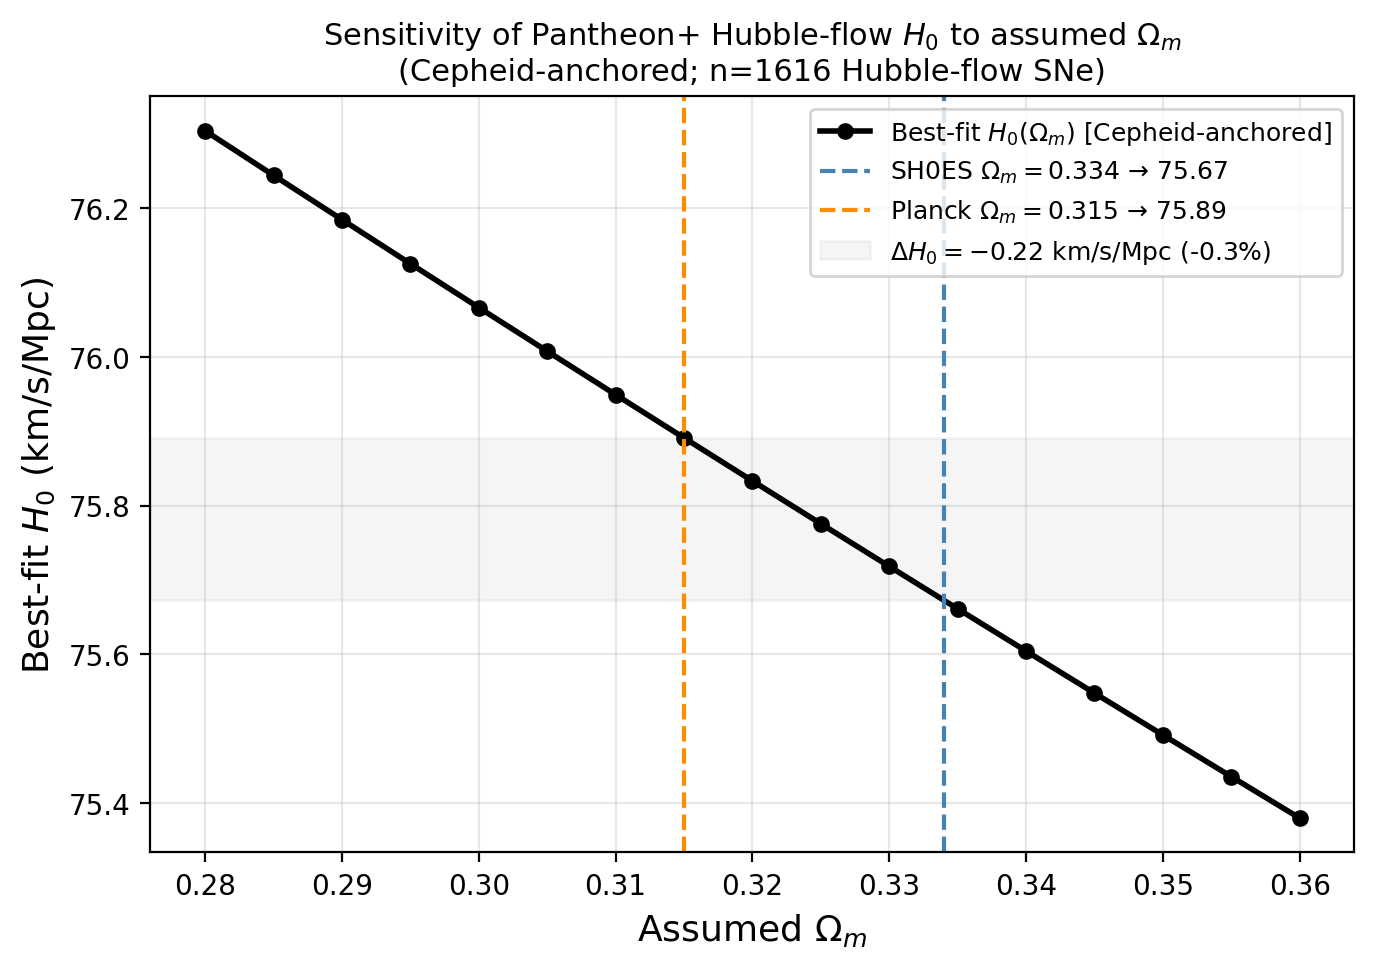
\includegraphics[width=\columnwidth]{refit_H0_vs_Om}
  \caption{Best-fit $H_0$ as a function of assumed $\Omega_m$,
    from the Cepheid-anchored refit of 1{,}616 Pantheon+ Hubble-flow SNe~Ia.
    Vertical dashed lines mark the Planck ($\Omega_m = 0.315$, orange)
    and SH0ES ($\Omega_m = 0.334$, blue) posterior best-fits.
    The shaded band shows the $|\Delta H_0| = 0.22$ km\,s$^{-1}$\,Mpc$^{-1}$
    sensitivity interval.}
  \label{fig:h0_vs_om}
\end{figure}

\begin{figure}
  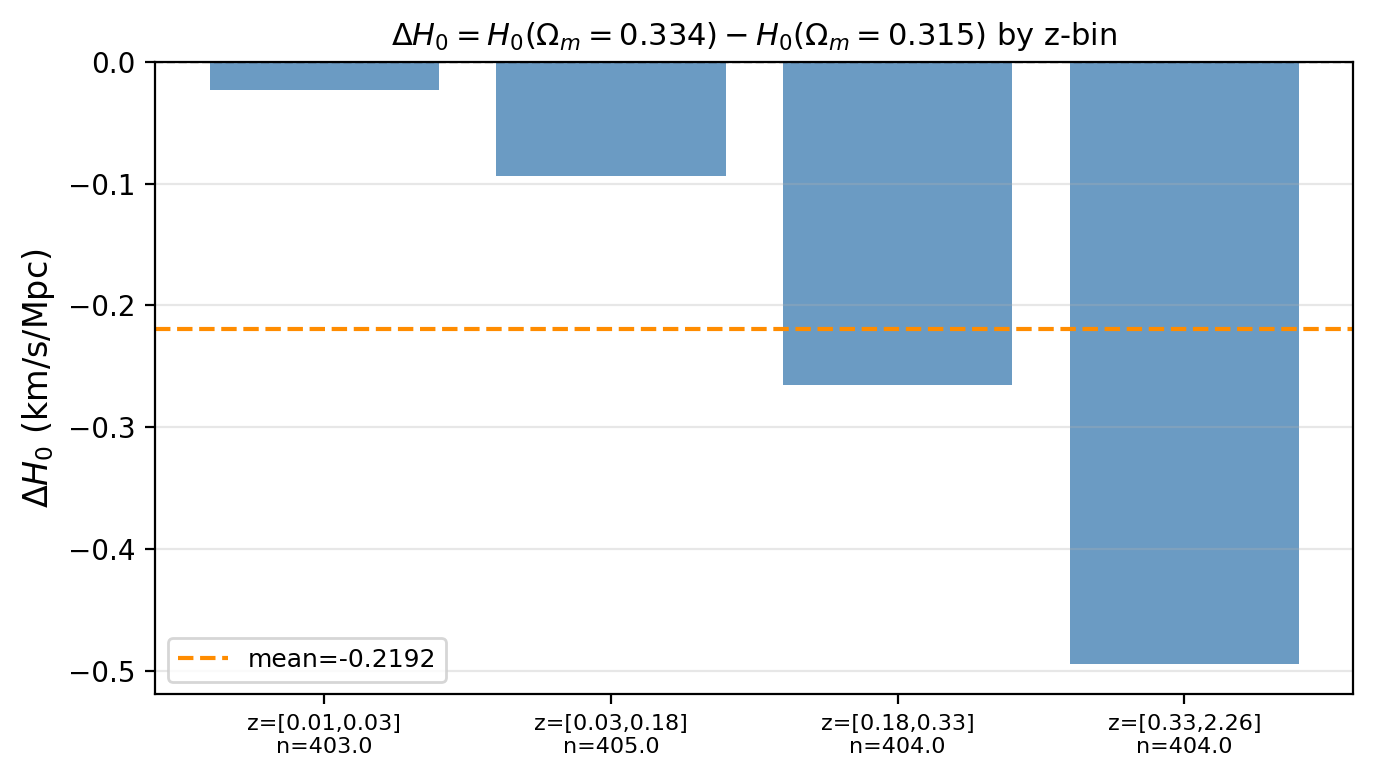
\includegraphics[width=\columnwidth]{zbin_deltaH0}
  \caption{$\Delta H_0 = H_0(\Omega_m=0.334) - H_0(\Omega_m=0.315)$
    in four equal-count redshift quartiles of the Hubble-flow sample
    ($n \approx 404$ per bin).
    The sign is uniform; the magnitude grows with redshift as the
    $\Omega_m$-dependent shape of $E(z)$ becomes increasingly important.
    The orange dashed line marks the mean ($-0.22$ km\,s$^{-1}$\,Mpc$^{-1}$).}
  \label{fig:zbin}
\end{figure}

\end{document}
